\section{Method} \label{sec:method}

\subsection{Data Construction} \label{sec:data}
%Ndapa: histroy is generally singular, 
We construct a dataset from Wikipedia edit history of person entities whose facts change between the year 2007 and 2012 (i.e., have at least one fact in YAGO KB \cite{suchanek2007yago} with a start or end time in this period). We obtain Wikipedia URLs of this set of entities $P$ from YAGO and crawl their article's revision history%, obtaining any revision their pages have between the year 2007 and 2012
. Given a person $p$, his/her Wikipedia revision history $R_p$ has a set of ordered dates $T_p$ on which revisions are made to his/her Wikipedia page (we consider date granularity). Each revision $r_{p, t} \in R_p$ is his/her Wikipedia page at date $t$ where $t \in T_p$. 

%For example, Ralph McInerny's Wikipedia page was consecutively revised on the dates of 11/20/2012, 12/26/2012 and 12/29/2012. We find the difference between the last revision to his page on 11/20/2012 and the first revision to his page on 12/29/2012 (since a page can be revised multiple times in a date). This difference\footnote[2]{http://en.wikipedia.org/w/index.php?title=Ralph\_McInerny \&type=revision\&diff=530257160\&oldid=523980632}, a HTML page obtained by ``compare selected revisions"  functionality in Wikipedia, is a document in our dataset. Using this method, we obtain 288,184 documents from revision histories of 16,909 Wikipedia entities. 

Each Wikipedia revision $r_{p, t}$ is a set of infobox slots $S_{p, t}$ and textual content $C_{p, t}$. Each infobox slot $s \in S_{p, t}$ is a quadruple, $\langle s_{att}$, $s_{value}$,  $s_{start}$, $s_{end} \rangle$ containing the attribute name (non-empty), the attribute value, and the start and end time for which this attribute-value pair is valid. 

A document $d_{p, t}$ in our data set is the \textit{difference}\footnote{a HTML document obtained by ``compare selected revisions"  functionality in Wikipedia} between any two consecutive revisions separated by at least a single date i.e., $d_{p, t} = r_{p, t+2} - r_{p, t}$, where $r_{p, t+2}$ is the \textit{first} revision on date $t+2$ and $r_{p, {t}}$ is the \textit{last} revision on date $t$ (as a page can be revised many times in a day). 

%Each document in our dataset 
A document $d_{p, t}$ is therefore %a \textit{difference} between $r_{p, t+2}$ and $r_{p, t}$, and is 
a set of infobox changes $\Delta S_{p, t}$ and textual changes $\Delta C_{p, t}$. Each slot change $\delta s \in \Delta S_{p, t} = \langle s_{att}$, $\delta s_{value}$,  $\delta s_{start}$, $\delta s_{end} \rangle$ %, where $\delta s_{value}$,  $\delta s_{start}$, or $\delta s_{end}$, whenever not empty, 
is prefixed with $+$ or $-$ to indicate whether they are added or deleted in $r_{p, t+2}$. Similarly, each text change $\delta c \in \Delta C_{p, t}$ is prefixed with $+$ or $-$ to indicate whether they are added or deleted% in $r_{p, t+2}$
. 

For example, in Figure \ref{fig:motivation}, a document $d_{kim,\ 05/23/2014} = r_{kim, 05/25/2014} - r_{kim, 05/23/2014}$ is a set of slot changes: $\langle\textsc{spouse}$, \textbf{$+$}\footnotesize ``Kanye West"\normalsize,  $+$\footnotesize ``2014"\normalsize, \footnotesize`` "\normalsize$\rangle$, $\langle\textsc{partner}$, $-$\footnotesize``Kanye West"\normalsize,  $-$\footnotesize``2012-present; engaged"\normalsize, \footnotesize`` "\normalsize$\rangle$ and a set of text changes: $+$\footnotesize``Kardashian and West were married in May 2014"\normalsize, $-$\footnotesize``She began dating West"\normalsize, $-$\footnotesize``they became engaged in October 2013"\normalsize.

For each $d_{p, t}$, we use $\Delta S_{p, t}$ to label the document and $\Delta C_{p, t}$ to extract features for the document. We label $d_{p, t}$ that has a new value or start time added to its infobox: $\langle s_{att}, +\delta s_{value}, *, *\rangle \in \Delta S_{p, t}$ or $\langle s_{att}, *, +\delta s_{start}, *\rangle$ $\in \Delta S_{p, t}$ with the label \textit{begin-}$s_{att}$ and label $d_{p, t}$ that has a new end time added to its infobox: $\langle s_{att}, *, *, +\delta s_{end}\rangle$ $\in \Delta S_{p, t}$ with the label \textit{end-}$s_{att}$. 

The label represents the state change that happens in $d_{p, t}$. For example, in Figure \ref{fig:motivation}, $d_{kim,\ 05/23/2014}$ is labeled with \textit{begin-spouse}% and \textit{end-partner}
. 

The revision history dataset that we make available for future research consists of all documents $d_{p, t}$, labeled and unlabeled, $\forall t \in T_p,\ t \in [01/01/2007,\ 12/31/2012]$, and $\forall p \in P$; a total of 288,184 documents from revision histories of 16,909 Wikipedia entities. Using our labeling process, we find that out of 288,184 documents, only 41,139 have labels (i.e., have their infobox updated with new values/start/end time). The distribution of labels in the dataset is skewed towards birth and death events as these are life events that happen to almost all person entities in Wikipedia. The distribution of labels in the dataset that we release can be seen in Figure~\ref{fig:distribution}. We show only labels that we evaluate in our task. 

\begin{figure*}[t]
\begin{center}
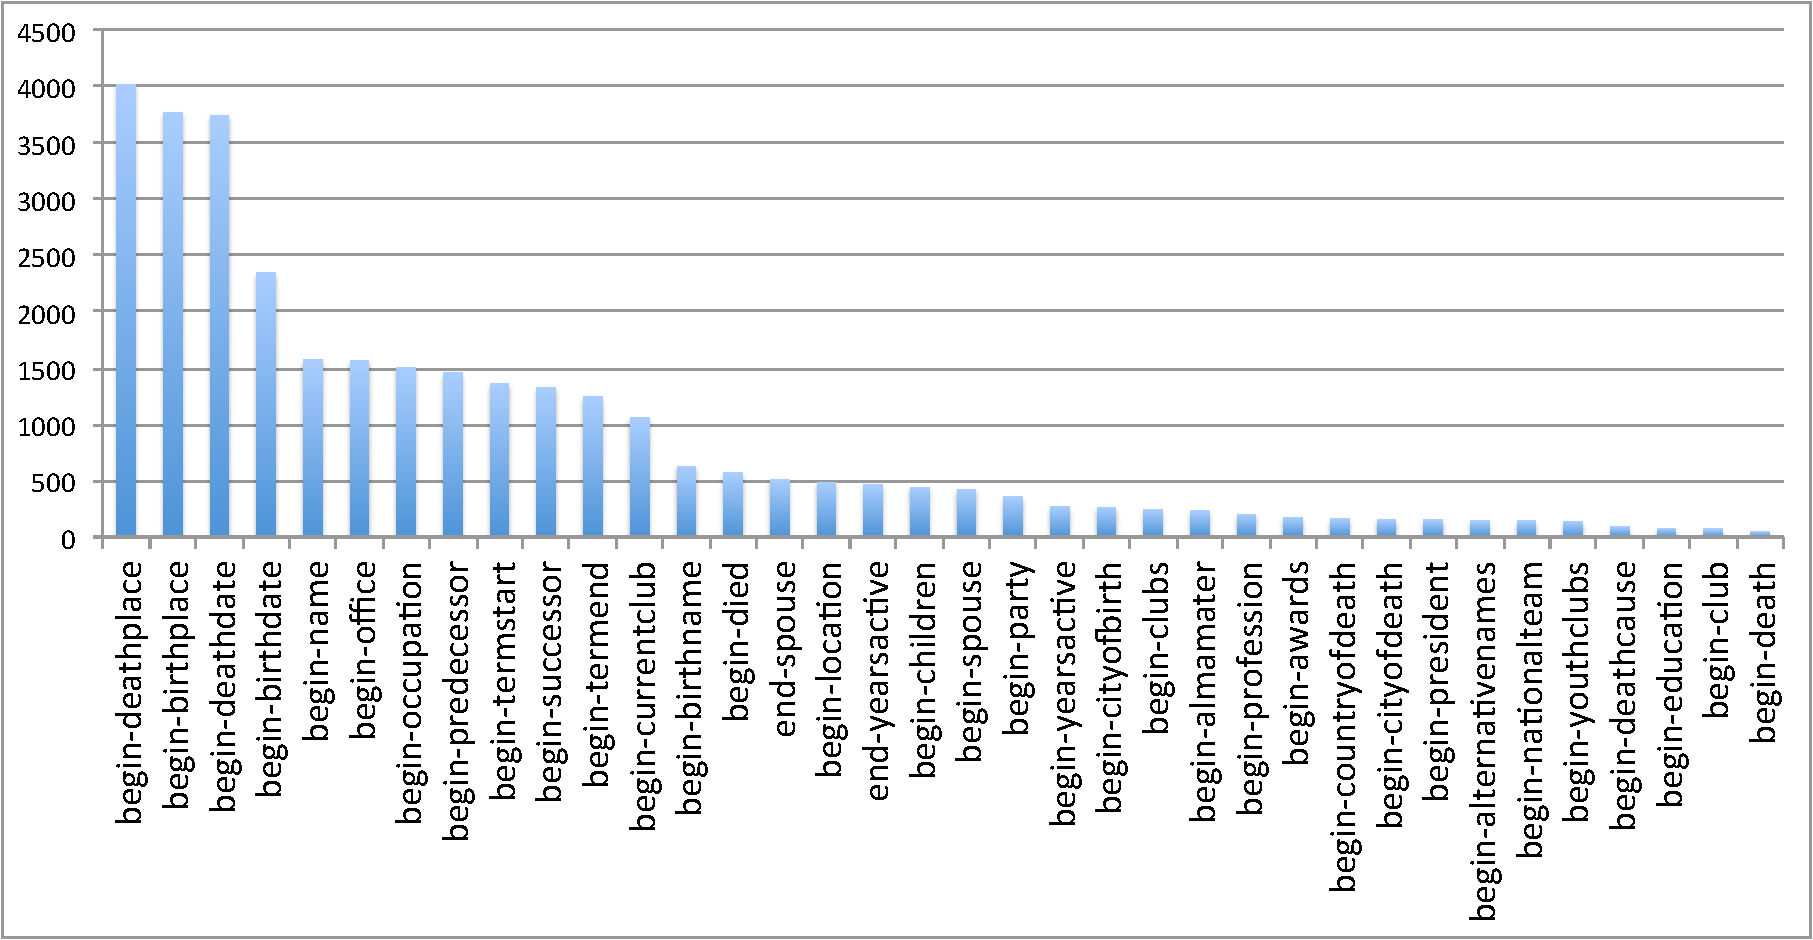
\includegraphics[width=15cm,keepaspectratio=true]{figures/distribution.pdf}
\caption{\label{fig:distribution} Distribution of labels we evaluate in our task in the revision history dataset.}
\end{center}
\end{figure*}

For our task of learning state changing verbs from this revision history dataset, for each labeled $d_{p,t}$, we extract as features, verbs (or verbs+prepositions) $v \in \Delta C_{p, t}$ that have its subject (or object) matches the Wikipedia entity $p$ \textit{and} its object (or subject resp.) matches an infobox value, start or end time: ($v_{subject}$, $v_{object}$) = (\scriptsize$arg1$\normalsize, \scriptsize$arg2$\normalsize) or ($v_{subject}$, $v_{object}$) = (\scriptsize$arg2$\normalsize,  \scriptsize$arg1$\normalsize), where \scriptsize$arg1$\normalsize = $p$ and $\langle s_{att}, $\scriptsize$arg2$\normalsize$, *, *\rangle$ or $\langle s_{att}, *, $\scriptsize$arg2$\normalsize$, *\rangle$ or $\langle s_{att}, *, *, $\scriptsize$arg2$\normalsize$\rangle$ $\in \Delta S_{p, t}$. We use Stanford CoreNLP \cite{manning-EtAl:2014:P14-5} to dependency parse sentences and extract the subjects and objects of verbs. We find that 27,044 out of the 41,139 \textit{labeled} documents contain verb edits, but only 4,735 contain verb edits with two arguments, where one argument matches the entity and another matches the value of the infobox change. We use the latter for our task, to improve the chance that the verb edits used as features are related to the infobox change. 

%  is the document's entity $p$ and whose object (\textit{arg2}) is any of its $\delta s$ value (or vice versa). We use 90\% of our labeled documents as training and test on the remaining 10\%. The task is to predict for each document, the label of the document given its verbs features. 

%We define an infobox attribute of an entity e.g., \textsc{spouse} to \textit{begin} when a new value or a begin time is added to the attribute slot and to \textit{end} when an end time is being added to the slot. Using regular expression to detect whether a new value, a start, or an end time is being added to infobox slots of a document, we automatically label each document with ``begin-\{attribute\_name\}" or ``end-\{attribute\_name\}". So a document that contains an addition of a new value in the \textsc{spouse} slot will be labeled ``begin-spouse", while a document that contains an addition of end time in the \textsc{spouse} slot will be labeled ``end-spouse". 

\subsection{Model}
We use a Maximum Entropy (\textsc{MaxEnt}) classifier\footnote{We use \textsc{Mallet} implementation of \textsc{MaxEnt}: http://mallet.cs.umass.edu/} given a set of training data = \{(\textbf{v}$_{d_{\ell}}$, y)\} where \textbf{v}$_{d_{\ell}} =$ ($v_1$, $v_2$, ... $v_{|V|}$) $\in R^{|V|}$ is the $|V|$-dimensional representation of a labeled document $d_{\ell}$ where $V$ is the set of all verbs in our training data, and $y$ is the label of $d_{\ell}$ as defined in \ref{sec:data}.

These training documents are used to estimate a set of weight vectors \textbf{w} = \{\textbf{w}$_1$, \textbf{w}$_2$, ... \textbf{w}$_{|Y|}$\}, \textbf{w}$_y$ $\in R^{|V|}$, one for each label $y \in Y$, the set of all labels in our training data. The classifier can then be applied to classify an unlabeled document $d_{\textit{u}}$ using: 
%\scriptsize
 \begin{equation}
	p(y|\textbf{v}_{d_{\textit{u}}}) = \frac{\mathrm{exp}  (\textbf{w}_{y} \cdot \textbf{v}_{d_{\textit{u}}})}{\sum_{y'} \mathrm{exp} (\textbf{w}_{y'} \cdot \textbf{v}_{d_{\textit{u}}})} \label{eqn:maxent}
\end{equation}
%\normalsize
\subsection{Feature Selection using Constraints}

While feature weights from the \textsc{MaxEnt} model allow us to identify verbs that are good features for predicting a particular state change label, our distantly supervised training data is inherently noisy. Changes to multiple infoboxes can happen within our revision.
We therefore   utilize constraints among state changes to select consistent verb features for each type of state change. 
%There is no guarantee that at any revision, the changed slots are related to the event being expressed in text. 
%For example, when death happens, birth-related information in the infobox may also be updated. This can lead to incorrect state change prediction. While using many distantly labeled data may help%reduce the effect of noise
%, improvements may be possible by leveraging constraints among state changes to select consistent verb features for each change. 

We use two types of constraints:  (1) mutual exclusion (\textit{Mutex}) which indicate that mutex state changes do not happen at the same time 
e.g., update on \textit{birthdate} should not \textit{typically} happen with update on \textit{deathcause}. Hence,  their state changing verbs should be different. %or that the start of \textit{spouse} is mutually exclusive with the end of \textit{spouse}. 
%A good \textit{base} verb\footnote{The verb root or base form of a verb} for one change e.g., ``marry" for \textit{begin-spouse} is therefore not a good feature for \textit{end-spouse} (mutex with \textit{begin-spouse}). 
(2) Simultaneous (\textit{Sim}) constraints which indicate that simultaneous state changes should \textit{typically} happen at the same time e.g., update on \textit{birthdate} should \textit{typically} happen with other birth-related updates such as \textit{birthplace}, \textit{birthname}, %\textit{birthcity}, 
etc. 
%A good base verb for one state change e.g., ``die" for \textit{begin-deathdate} is therefore a good feature for \textit{begin-deathdate}'s simultaneous changes: \textit{begin-deathplace}, \textit{begin-deathcause}, etc. 
We manually specified these two types  of  constraints to all pairs infoboxes where they apply. We have 10 mutex constraints and 23 simultaneously updated constraints.
%Labels that share the same prefix such as \textit{begin-birth*} have simultaneous constraints while labels that share the same suffix but different prefix such as \textit{begin-spouse} and \textit{end-spouse} or \textit{begin-yearsactive} and \textit{end-yearsactive} have mutually exclusive constraints.

Given a set of constraints, a set of labels $Y$, and a set of base verbs\footnote{The verb root or base form of a verb (after removing preposition)} $B$ in our training data, we solve a Mixed-Integer Program (MIP) for each base verb $b \in B$ to estimate whether $b$ should be a feature for state change $y \in Y$. 

We obtain label membership probabilities \{$P(y | b) = count(y, b) / \sum_{y'} count(y', b) $\} from our training data. The MIP takes the scores $P(y | b)$ and constraints as input and produces a bit vector of labels \textbf{a}$_{b}$ as output, each bit  $a_{b}^{y} \in \{0,\ 1\}$ represents whether or not $b$ should be a feature for $y$.

The MIP formulation for a base verb $b$ is presented by Equation \ref{eqn:mip}. For each $b$, this method tries to maximize the sum of scores of selected labels, after penalizing for violation of label constraints. Let $\zeta_{y, y'}$ be slack variables for \textit{Sim} constraints, and $\xi_{y, y'}$ be slack variables for \textit{Mutex} constraints. 

Solving MIP per base verb is fast; we reduce the number of labels considered per base verb i.e., we only consider a label $y$ to be a candidate for $b$ if $\exists\ v_i \in V$ s.t. $w_y^i > 0$ and $b$ = base form of $v_i$. %Then, we need to only solve MIP for base verbs that have non-empty candidate labels. 

After we output \textbf{a}$_b$ for each $b$, we select features for each label. We only select a verb $v_i$ to be a feature for $y$ if the learned weight $w_y^i > 0$ and $a_b^{y} = 1$, where $b$ = the base form of $v_i$. Essentially for each label, we select verb features that have positive weights and are consistent for the label.

\scriptsize
\begin{equation}
\begin{aligned}
& \operatorname*{maximize}_{\textbf{a}_b,\ \zeta_{y, y'},\ \xi_{y, y'}} 
& & \bigg( \sum_{y} a_{b}^{y}\ *\ P(y | b)\ - \sum_{\langle y, y'\rangle \in Sim} \zeta_{y, y'}\ - \\
& & & \sum_{\langle y, y'\rangle \in Mutex} \xi_{y, y'}\bigg) \\ 
& \text{subject to} & & \big(a_{b}^{y} - a_{b}^{y'}\big)^2 \leq \zeta_{y, y'},\ \ \ \forall \langle y, y'\rangle \in Sim \\
& & & a_{b}^{y} + a_{b}^{y'} \leq 1 + \xi_{y, y'},\ \ \ \forall \langle y, y'\rangle \in Mutex \\
& & & \zeta_{y, y'},\ \xi_{y, y'} \geq 0,\ a_{b}^{y} \in \{0, 1\},\ \ \ \forall y, y'
\label{eqn:mip}
\end{aligned}
\end{equation}
\normalsize
